\documentclass{vie16}
\usepackage{wrapfig}
\usepackage{float}
\usepackage{amsmath}
\usepackage[table,xcdraw]{xcolor}
\usepackage{booktabs}
\usepackage{multirow}
\usepackage{adjustbox}
\usepackage{subfigure}

% Path to figures
\graphicspath{{Fig/}}

% COMENTAR ANTES DE SUBMETER!
% Comando temporarios
\usepackage{color}
\usepackage[normalem]{ulem}
\newcommand{\new}[1]{\textcolor{blue}{#1}}
\newcommand{\old}[1]{\textcolor{MyDarkViolet}{\sout{#1}}}
\newcommand{\att}[1]{\textcolor{red}{#1}}
\newcommand{\js}[1]{\textcolor{darkgreen}{#1}}
\newcommand{\obs}[1]{\textcolor{orange}{#1}}
\definecolor{MyDarkViolet}{rgb}{0.602,0,0.602}
\definecolor{orange}{RGB}{255,127,0}
\definecolor{darkgreen}{RGB}{0,127,0}

% For pdf hyperlinks
\usepackage{hyperref} \hypersetup{colorlinks=true}
\hypersetup{citecolor=blue} \hypersetup{pdftitle={Global
optimization for AVO inversion: analysis of ray theory based
forward modelling algorithm}}
\hypersetup{pdfauthor={W.~C.~Ferreira, F.~Hilterman,
L.~A.~Diogo, H.~B.~Santos, J.~Schleicher and A.~Novais}}
% For making a print without color links
\hypersetup{linkcolor=black,citecolor=black,filecolor=black,urlcolor=black}
\hypersetup{linkcolor=blue,citecolor=blue,filecolor=blue,urlcolor=blue}
\usepackage{url}


% Criar fluxogramas
\usepackage[latin1]{inputenc}
\usepackage{tikz}
\usetikzlibrary{shapes,arrows} 

% definindo blocos para o fluxograma
\tikzstyle{decision} = [diamond, draw, fill=blue!20, text width=6.5em, text 
badly centered, node distance=3cm, inner  sep=0pt]
\tikzstyle{decisionmi} = [diamond, draw, fill=blue!20, 
text width=1.5em, text badly centered, node distance=3cm, inner sep=0pt]
\tikzstyle{block} = [rectangle, draw, fill=blue!20, 
text width=16em, text centered, rounded corners, minimum height=4em]
\tikzstyle{blockm} = [rectangle, draw, fill=blue!20, 
text width=6em, text centered, rounded corners, minimum height=4em]
\tikzstyle{blockmg} = [rectangle, draw, fill=blue!20, 
text width=10em, text centered, rounded corners, minimum height=2em]
\tikzstyle{blockmi} = [rectangle, draw, fill=blue!20, 
text width=3em, text centered, rounded corners, minimum height=2em]
\tikzstyle{blockf} = [rectangle, draw, fill=blue!20, 
text width=16em, text centered, rounded corners, minimum height=4em]
\tikzstyle{line} = [draw, -latex']
\tikzstyle{cloud} = [draw, ellipse,fill=blue!20, node distance=3cm,
minimum height=3em]
\tikzstyle{cloudr} = [draw, ellipse,fill=blue!20, node distance=3cm,
minimum height=3em]

\begin{document}
\title{Global optimization for AVO inversion: analysis of ray
theory based forward modelling algorithm}
\author{W.~C.~Ferreira, F.~Hilterman, L.~A.~Diogo, H.~B.~Santos,
J.~Schleicher and A.~Novais}
\maketitle

\begin{abstract}
Amplitude Variation with Offset (AVO) inversion provides
estimates of the P-wave velocity, S-wave velocity and density of
the stratified medium. A global optimization technique was
selected for the inversion due to the multi-parametric behaviour
of the AVO inversions which are strongly affected by the initial
estimate of the model rock properties.  An analysis to verify
the dependency between P-wave, S-wave velocity and density in
the recovered parameters was also performed using empirical
relations as constraints. In inversion schemes, the forward
modelling is often the most time consuming process. To reduce
computation time, we have implemented a genetic algorithm and a
\textit{table-based} ray-theory algorithm to allow us to
implement a large amount of models in the global search. Our
results show that the genetic algorithm was capable to recover
the physical parameters with good agreement for the examples
using the empirical constraints, but was also capable of
converging to solutions which were far from the correct answer,
but were good answers to explain the observed dataset. The
forward modelling algorithm has shown excellent performance to
be used in global optimization schemes allowing the use of a
large number of members in the population of the genetic
algorithm.
\end{abstract}

\newpage
\section{Introduction}
The methodology of AVO has been widely used in the industry as a
direct hydrocarbon indicator. In order to provide a quantitative
interpretation, AVO inversion to the rock properties has been
exploited. In forward model, the computation of the reflection
amplitude as a function of incident angle (offset) is
classically attributed to \cite{Zoeppritz1919} and
\cite{Knott1899} for plane waves. For the reverse model,
\cite{Rosa1976} derived and verified the ill-posed nature of the
inversion of Zoeppritz equations for rock properties, meaning
that we have multiple combinations of input to produce the same
output.  Moreover, \cite{Stoffa1991}, \cite{Mallick1995} and
others suggest global optimization schemes to treat the AVO
inversion due to its multi-parametric formulation which implies
a very complex solution space with many local minima, which
makes it difficult to find correct solutions. However, the
process of global optimizations requires many forward models
which increase considerably the time of computation. Many of the
works published in literature use forward modelling algorithms
based on the wave equation, which demands great computational
power. This study is based on the premise that unconsolidated
sediments with small rock-property changes between layers can be
modeled with ray theory without a loss of resolution. For
computational ease we have developed a forward modeling
algorithm called \textit{table-based ray theory} in order to
speed up the computation of synthetics seismograms for global
optimization.  The genetic algorithm was based on findings of
\cite{Stoffa1991} and \cite{Sen1992} and used the
\cite{Gardner1974} and \cite{Castagna1985} empirical
relationships as constrains to verify the dependency among the
parameters.

\section{Synthetic common-midpoint seismogram: forward
modelling} 

The forward modelling algorithm implemented is the
\textit{table-based ray tracing}. The Earth model assumed is the
isotropic layer model where the parametric equations are
used to compute the two-way traveltimes and offset as a function
of a constant ray parameter \citep{Geyer1959}, the
equations are given by
%!
\begin{eqnarray} x & = & 2\sum_{i=1}^{n} \frac {h_{i}pv_{i}} {(1
		- p^{2}v_{i}^{2})^{1/2}} \ ,\label{eq.x} \\ t & = &
		2\sum_{i=1}^{n} \frac {h_{i}} {v_{i}(1 -
		p^{2}v_{i}^{2})^{1/2}} \ , \label{eq.t} \end{eqnarray}
%
where $h_{i}$, $v_{i}$ and $p$ are, respectively, the
layer thickness, velocity and ray parameter which is
defined by
%!
\begin{equation}
p = \frac{\sin(\theta_{i})}{v_{i}}\ ,\label{eq.p}
\end{equation}
%!
where $\theta_i$ is the angle between the seismic ray and the
vertical in the $i$-th layer. Using a sonic log or other
vertical velocity information, three different
two-dimensional tables (\textit{offset, traveltime and
reflection coefficient}) are built starting with equations
\ref{eq.x} and \ref{eq.t}.

To start the process, the P-wave velocity as a function of depth
is transformed to time. The same applies to the S-wave velocity
and density. For the 2D traveltime table, there are 90 columns
associated with the ray parameter when the incident angle in the
first medium varies from $0\degree$ to $89\degree$. The rows are
associated with the $t_{o}$ times in increments of the time
sample interval. Now, the 2D tables for offset and traveltime
can easily be determined using equations \ref{eq.x} and
\ref{eq.t} respectively. Since the velocity function is sampled
in equal increments of the sample rate the same way the 2D
tables are, the computation of the incident angle for each cell
in the 2D table is possible with equation \ref{eq.p}. With the
incident angle known, the next step is to compute the 2D table
of reflection coefficients at each interface. This was
accomplished with Shuey's approximation \citep{Shuey1985} given by
%!
\begin{equation}
R_{P} (\phi) = A + B\sin^{2}(\theta) + C\sin^{2}(\theta)\tan^{2}(\theta)
\ , \label{eq.shuey}
\end{equation}
%!
where $\phi$ is the incident angle, $\theta$ is the average of
the incident and transmitted angles, and the terms $A$, $B$ and
$C$ are defined as
%?!
\begin{equation}
\begin{split}
A & = \frac{1}{2} \left(\frac{\triangle V_{P}}{V_{P}}     +
\frac{\triangle \rho}{\rho}     \right)\ , \\
B & = \frac{1}{2} \frac{\triangle V_{P}}{V_{P}}  - 2\left(\frac{
V_{S}}{V_{P}}\right)^{2}  \left(\frac{2\triangle V_{S}}{V_{S}} +
\frac{\triangle \rho}{\rho}\right)   \ , \\
C & = \frac{1}{2} \left(\frac{\triangle V_{P}}{V_{P}} \right) \ .
\end{split}
\end{equation}
%!
In these expressions, $\triangle V_{P} = V_{P2} - V_{P1}$,
$\triangle V_{S} = V_{S2} - V_{S1}$, $\triangle \rho = \rho_{2}
- \rho_{1}$, where $V_{P}$, $V_{S}$ and $\rho$ are arithmetic
averages for P-wave and S-wave velocities and the density.

Finally, in order to build the common-midpoint (CMP) synthetic
seismogram, we define which are the offsets to model and start a
search row-by-row inside the \textit{offset table} looking for
the requested offsets.  Once the cell is found for the specified
offset, we go into the same cell position inside the
\textit{traveltime} and \textit{reflectivity tables} to place
the reflection coefficient from that position in the correct
time arrival inside the trace.

The algorithm is simple and provides the opportunity to be
easily adapted to study more complex effects such as the stretch
in normal moveout (NMO) correction, NMO without stretch
(ray-trace NMO correction), array effects which affect the
amplitude of the wave received by the streamer, easily
extraction of AVO attributes, polar anisotropic media, etc.
 
\section{Global optimization approach: Genetic Algorithm}
\begin{wrapfigure}{l}{0.49\textwidth}
 \centering
 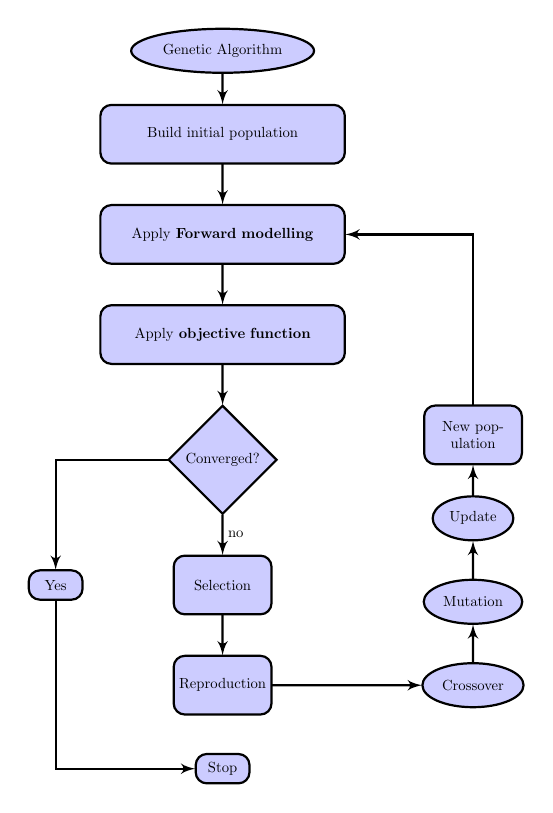
\begin{tikzpicture}[thick,scale=0.53, every 
 node/.style={scale=0.53},node distance = 2.4cm, auto]
    % Place nodes
    \node [block] (init) {Build initial population};
    \node [cloud, above of=init, node distance=2cm] (expert) {Genetic 
    Algorithm};
    \node [block, below of=init] (identify) {Apply \textbf{Forward modelling}};
    \node [blockf, below of=identify] (pop) {Apply \textbf{objective 
    function}}; 
    \node [decision, below of=pop] (evaluate) {Converged?};
    \node [blockm, below of=evaluate, node distance=3cm] (select) 
    {Selection};
    \node [blockm, below of=select] (reprod) {Reproduction};
    \node [cloudr, right of=reprod, node distance=6cm] (crossover) 
    {Crossover};
    \node [cloudr, above of=crossover, node distance=2cm] (mutation) 
    {Mutation};
    \node [cloudr, above of=mutation, node distance=2cm] (update) {Update};
    \node [blockm, above of=update, node distance=2cm] (newpop) {New 
    population};
    \node [blockmi, below of=reprod, node distance=2cm] (stop) {Stop};
    \node [blockmi, left of=select, node distance=4cm] (sim) {Yes};

    % Draw edges
    \path [line] (init) -- (identify);
    \path [line] (identify) -- (pop);
    \path [line] (pop) -- (evaluate);
    \path [line] (expert) -- (init);
    \path [line] (evaluate) --  node {no} (select);
    \path [line] (select) -- (reprod);
    \path [line] (reprod) -- (crossover);
    \path [line] (crossover) -- (mutation);
    \path [line] (mutation) -- (update);
    \path [line] (update) -- (newpop);  
    \path [line] (newpop) |- (identify);
    \path [line] (evaluate) -| (sim);
    \path [line] (sim) |- (stop);
\end{tikzpicture}
\caption{Flowchart of the genetic algorithm.}
% implemented in FORTRAN 77/90.}
\label{fig.fluxo}
\end{wrapfigure}

The genetic algorithm (Figure~\ref{fig.fluxo}) is a technique used to perform 
global optimizations based in the natural selection \citep{Holland1975}. In 
order to simulate this process, the algorithm constantly modify the initial 
pseudo-random population in order to reach local minima positions. 
Initially, each member of the pseudo-random population is a potential 
solution to the problem and after some iterations the genetic algorithm will 
guide the population to the best fit positions.

The algorithm needs to \textit{select} a percentage of the population to start 
the reproduction scheme where the \textit{crossover} and the 
\textit{mutation} are the two classic techniques to exchange genetic 
information between the members and also randomly change the genetic 
information to provide exploration of the solution space. In order to select 
the members of the population we need to measure the fitness between each 
potential solution and the data we want to optimize. The objective function 
used was proposed by \cite{Porsani2000} and is given by
%!
\begin{equation}
h = \frac{2y^{T} x} {y^{T}y + x^{T}x} \ ,
\label{eq.Porsani}
\end{equation}
%!
where, $x$ e $y$ are respectively the observed data and modelled data in 
the time domain and  $x^{T}$, $y^{T}$ are their transposes. In order to 
constrain the inverse problem due to the dependency between S-wave 
velocity and density with P-wave velocity, it was used the Gardner 
\citep{Gardner1974} and Castagna \citep{Castagna1985} relations 
to write S-wave and density as a function of P-wave.

\section{Results}
A synthetic model was used in order to verify the global optimization 
method for AVO inversion and its relationships with the prior informations 
(\cite{Gardner1974} and \cite{Castagna1985} constrains) and also to 
analyse the performance of the forward modelling algorithm proposed. The 
physical parameters for the synthetic model is described in the 
Table~\ref{tab.model}. The thickness between the two inner layers was 
chosen to be small enough to allow interaction between the wavelets.

% Please add the following required packages to your document preamble:
% \usepackage{booktabs}
% \usepackage[table,xcdraw]{xcolor}
% If you use beamer only pass "xcolor=table" option, i.e. 
%\documentclass[xcolor=table]{beamer}
%\begin{table}[]
%\centering
%\caption{My caption}
%\label{my-label}
\begin{wraptable}{l}{0.49\textwidth}
\caption{Model parameters.}
\begin{adjustbox}{max width=0.46\textwidth}
\label{tab.model}
\begin{tabular}{@{}
>{\columncolor[HTML]{FFFFFF}}c 
>{\columncolor[HTML]{FFFFFF}}c 
>{\columncolor[HTML]{FFFFFF}}c 
>{\columncolor[HTML]{FFFFFF}}c 
>{\columncolor[HTML]{FFFFFF}}c @{}}
\toprule
\textbf{Layers} & \textbf{\begin{tabular}[c]{@{}c@{}}Thickness\\ 
(m)\end{tabular}} & \textbf{\begin{tabular}[c]{@{}c@{}}Vp \\ 
(m/s)\end{tabular}} & \textbf{\begin{tabular}[c]{@{}c@{}}Vs\\ 
(m/s)\end{tabular}} & \textbf{\begin{tabular}[c]{@{}c@{}}Density\\ 
(g/cc)\end{tabular}} \\ \midrule
1 & 1000 & 2000 & 551.72 & 1.5381 \\
2 & 50 & 2800 & 1241.38 & 1.6731 \\
3 & 50 & 2300 & 810.34 & 1.5928 \\
4 & 500 & 3000 & 1413.80 & 1.7022 \\ \bottomrule
\end{tabular}
%\end{table}
\end{adjustbox}
\end{wraptable}

The parameters used in the forward modelling shown in 
Figure~\ref{fig.fluxo} was a zero phase Ricker wavelet with central frequency 
in 40~Hz and discretization time of 2~ms. In order to perform the global 
optimization the CMP gathers have to be previously corrected from the NMO.
%!
The parameters used in the \textit{genetic algorithm} is given by 
\textit{selection rate} of $50\%$, $P_{mutation}$~=~0.1, 
$P_{update}$~=~0.47, $P_{crossover}$~=~0.90,~1000 members in the 
population and a convergence criterion of 200 iterations.

In the following results only the parameters from the fourth layer of the 
model from Table~\ref{tab.model} will be shown in more detail due to the 
limit of space. The Figure~\ref{fig2} shows the evolution of the genetic 
algorithm solutions for the P-wave velocity parameter in the fourth layer 
when running with and without the \cite{Gardner1974} and 
\cite{Castagna1985} constrains. As we can see in Figure~\ref{fig2-with}, 
after few iterations the algorithm is already guiding all the members in the 
population close to the correct position in the solution space.
%!
However, the Figure~\ref{fig2-without} shows that even with the lack of 
additional constrains to restrict the solutions, the algorithm is leading the 
population to particular solutions which are not so close to the correct one 
but are good answers to the inverse problem as we can see in 
Table~\ref{tab.recovered}.

\begin{figure}[H]
%\subfigcapskip-5pt
\subfigtopskip-5pt
\subfigbottomskip0pt
\subfigure[]{
    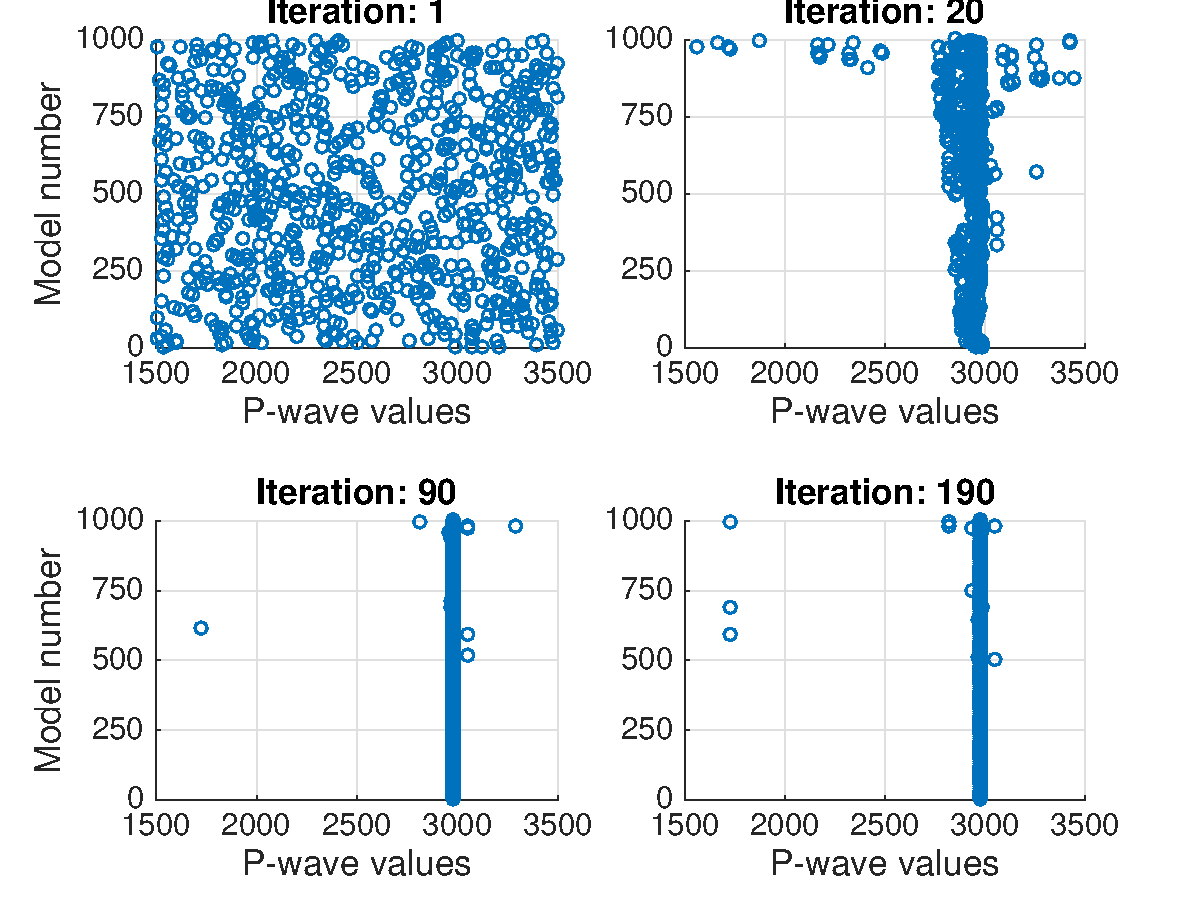
\includegraphics[width=0.49\textwidth]{evol-sol-constrains-edit}
    \label{fig2-with} 
}
\subfigure[]{
    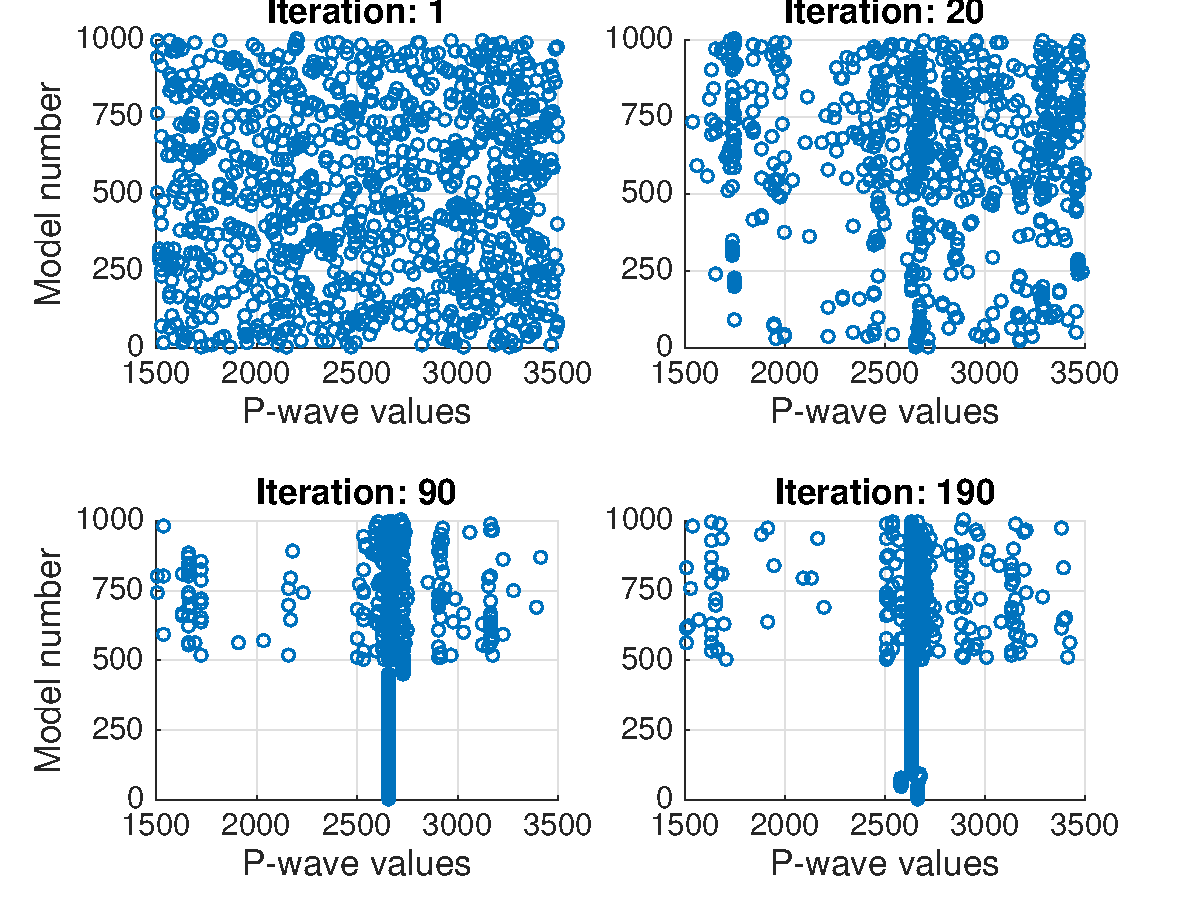
\includegraphics[width=0.49\textwidth]{evol-sol-no-constrains-edit}
    \label{fig2-without} 
}
\caption{Evolution of the genetic algorithm solutions for the P-wave 
velocity parameter in the fourth layer when running with \subref{fig2-with} 
and without \subref{fig2-without} the \cite{Gardner1974} and 
\cite{Castagna1985} constrains.
}
%% Wanderson, assim que tivermos as figuras finais a gente tem que voltar 
%%aqui e melhorar a descricao
\label{fig2}
\end{figure}

In Table~\ref{tab.recovered} we can see the values for the best model 
recovered with and without the constrains in the parameters. The algorithm 
performed 301.000 forward modelling in 36 minutes. Even with more than 
$20\%$ of relative error in average, the best model recovered without the 
constrains still produce a very similar CMP gather as we can verify by the 
correlation coefficient value.
%%
%% Wanderson, vc fez a tab no site que eu te indiquei?

% Please add the following required packages to your document preamble:
% \usepackage{booktabs}
% \usepackage{multirow}
\begin{table}[h!]
%\caption{Recovered parameters of the model in the fourth layer when 
%running with and without the Gardner and Castagna constrains.}
\caption{Recovered parameters of the model with and without constrains.}
\begin{adjustbox}{max width=\textwidth}
\label{tab.recovered}
\begin{tabular}{@{}cccccc@{}}
\toprule
\multirow{2}{*}{\textbf{Parameters}} & \multirow{2}{*}{\textbf{Synthetic 
Model}} & \multicolumn{2}{c}{\textbf{\begin{tabular}[c]{@{}c@{}}Recovered 
Model\\ (with constrains)\end{tabular}}} & 
\multicolumn{2}{c}{\textbf{\begin{tabular}[c]{@{}c@{}}Recovered Model\\ 
(without constrains)\end{tabular}}} \\ \cmidrule(l){3-6} 
 &  & \textbf{Parameters} & \textbf{Relative Error (\%)} & \textbf{Parameters} 
 & \textbf{Relative Error (\%)} \\ \cmidrule(r){1-2}
\multirow{4}{*}{\begin{tabular}[c]{@{}c@{}}P-wave\\ (m/s)\end{tabular}} & 
2000 & 2000 & 0.00 & 2002 & -0.10 \\
 & 2800 & 2788 & 0.43 & 2699 & 3.61 \\
 & 2300 & 2280 & 0.87 & 2394 & -4.09 \\
 & 3000 & 2971 & 0.97 & 2658 & 11.40 \\
\cmidrule{2-6}
\multirow{4}{*}{\begin{tabular}[c]{@{}c@{}}S-wave\\ (m/s)\end{tabular}} & 
551.72 & 552.71 & -0.07 & 778 & -41.01 \\
 & 1241.38 & 1231 & 0.84 & 1327 & -6.90 \\
 & 810.34 & 793 & 2.14 & 1106 & -36.49 \\
 & 1413 & 1389 & 1.75 & 1358 & 3.95 \\
\cmidrule{2-6}
\multirow{4}{*}{\begin{tabular}[c]{@{}c@{}}Density\\ (g/cc)\end{tabular}} 
& 1.5381 & 1.538 & 0.01 & 1.1408 & 25.83 \\
 & 1.6731 & 1.671 & 0.13 & 1.2932 & 22.71 \\
 & 1.5928 & 1.589 & 0.24 & 1.1466 & 28.01 \\
 & 1.7022 & 1.698 & 0.25 & 1.4416 & 15.31 \\
\cmidrule{1-6}
\multicolumn{1}{l}{\textbf{Correlation Coef.}} & 1 & 
\multicolumn{2}{c}{0.999887645} & \multicolumn{2}{c}{0.999847412} \\ 
\bottomrule
\end{tabular}
\end{adjustbox}
\end{table}

\section{Conclusions}
The forward modelling algorithm presented has shown excellent potential to 
be used in global optimization schemes by providing good performance in a 
regular computer. The constrains are also helpful in the process however the 
result without constrains indicate that we can still converge to particular 
results. The genetic algorithm will be formulated inside the Bayesian 
framework to provide solid statistical informations about the distribution of 
the solutions during the iterations. It is expected to be able to visualize 
distinguishable concentration of particular solutions which could be useful 
to determine possible scenarios for the recovered parameters. Finally, for 
future work in this project will also introduce errors in the models and an 
application to real data to verify the reliability of this technique.

\section{Acknowledgements}
This research was supported by the Brazilian research agencies CAPES, CNPq, 
FAPESP and FINEP. The first author W. C. Ferreira thanks to CAPES for the 
Science Without Borders fellowship, Geokinetics and the Allied Geophysical 
Laboratories. H. B. Santos is grateful to CGG-Brazil and Petrobras for his 
fellowships. Additional support for the authors was provided by the 
sponsors of the \textit{Wave Inversion Technology (WIT) Consortium}.

\bibliography{EAGE2016}
\end{document} 